\documentclass[a4paper]{article}

%% Language and font encodings
\usepackage{polski}
\usepackage[utf8]{inputenc}
\usepackage[T1]{fontenc}
\usepackage{pdfpages}
\usepackage{indentfirst}

% Adjust penalties
\brokenpenalty=1000
\clubpenalty=1000
\widowpenalty=1000

%% Sets page size and margins
\usepackage[a4paper]{geometry}

%% Useful packages
\usepackage{amsmath}
\usepackage{graphicx}
\usepackage[colorlinks=true, allcolors=blue]{hyperref}
\usepackage{booktabs}
\usepackage{cancel}
\usepackage{tikz}

\usepackage{float}

\renewcommand\thesection{\arabic{section}.}
\renewcommand\thesubsection{\arabic{section}.\arabic{subsection}.}
\renewcommand\thesubsubsection{\arabic{section}.\arabic{subsection}. \arabic{subsubsection}.}

% The following commands are not supported in PSTricks at present
% We define them conditionally, so when they are implemented,
% this pgf file will use them.
\ifx\du\undefined
  \newlength{\du}
\fi
\setlength{\du}{15\unitlength}

\newcommand{\Vsp}[1]{\vtop to #1 {}}
\newcommand{\Hsp}[1]{\hbox to #1 {}}
\newcommand{\Small}{\scriptsize}

\title{Sprawozdanie nr 3}
\date{}


\begin{document}

\begin{center}
\begin{tabular}{|p{5.5cm}|l|l|c|}
    \hline
	% Row 1.1  
	    Wydział \Vsp{4mm} &
	    \multicolumn{1}{|l}{Dzień} &
	    poniedziałek $17^{15} - 19^{30}$ &
	    Nr zespołu \\
	% Row 1.2
	    \mbox{\small{Matematyki i Nauk Informatycznych}} &
	    \multicolumn{1}{|l}{Data}  &
	    &
	    \multicolumn{1}{c|}{\Large{18}} \\
    
    \hline
	% Row 2.1 
	    Nazwisko i Imię: &
	    \Small Ocena z przygotowania &
	    \Small Ocena ze sprawozdania &
	    \Small Ocena Końcowa \\
	% Rows 2.2-2.4
	    1. Jasiński Bartosz & & &\\
	    2. Sadłocha Adrian & & & \\
	    3. Wódkiewicz Andrzej & & & \\

    \hline
    % Row 3.1
	    \multicolumn{2}{|l|}{Prowadzący \Vsp{4mm}} &
	    \multicolumn{2}{|l|}{Podpis prowadzącego} \\  
    % Row 3.2
    	\multicolumn{2}{|l|}{dr inż. Mateusz Szeląg} &
    	\multicolumn{2}{|l|}{} \\    	
    \hline
\end{tabular}
\label{pieczatka}
\end{center}

{\let\newpage\relax\maketitle}  % stolen from: https://tex.stackexchange.com/questions/86249/maketitle-text-before-title
\setcounter{secnumdepth}{2}


\section{Opis ćwiczenia}


\subsection{Wstęp teoretyczny}

\subsection{Układ pomiarowy}

\section{Pomiary i obliczenia}

\subsection{Wyznaczenie objętości kulek}

W celu wyznaczenia objętości kulek dokonaliśmy 10 pomiarów średnicy za pomocą śruby mikrometrycznej.
Wyniki przedstawiliśmy w tabeli \ref{kulki_srednica}.

\begin{table}[h!]
	\centering
	\begin{tabular}{lrr}
		\toprule
		L.p. &  średnica (mm) &  promień (mm) \\
		\midrule
		1 &           2.77 &         1.385 \\
		2 &           2.78 &         1.390 \\
		3 &           2.78 &         1.390 \\
		4 &           2.77 &         1.385 \\
		5 &           2.77 &         1.385 \\
		6 &           2.76 &         1.380 \\
		7 &           2.77 &         1.385 \\
		8 &           2.78 &         1.390 \\
		9 &           2.78 &         1.390 \\
		10 &           2.77 &         1.385 \\
		\midrule
		Średnia: & 2.773 & 1.3865 \\
		Odchylenie standardowe: & 0.006749 & 0.003375 \\
		\bottomrule
	\end{tabular}
	\caption{Wyniki 10 pomiarów średnicy kulek}
	\label{kulki_srednica}
\end{table}

Średnia wartość średnicy wynosi $d = 2.773$ mm, zaś średnia wartość promienia $r = \frac 1 2 \cdot 2.773 = 1.3865$ mm.

Oznaczmy przez $\Delta d$ -- niepewność wynikającą z wykorzystania śruby mikrometrycznej,
zaś przez $\Delta d_e$ -- niepewność eksperymentatora.

W przypadku użytej przez nas śruby mikrometrycznej $\Delta d = 0.01$ mm.
Za niepewność eksperymentatora przyjęliśmy połowę najmniejszej podziałki, tj. $\Delta d_e = 0.005$ mm.

Zatem niepewność pomiarowa typu B wynosi:

\begin{align*}
	u_b(d) &= \sqrt{\left(\frac{\Delta d}{\sqrt 3}\right)^2 + \left(\frac{\Delta d_e}{\sqrt 3}\right)^2} \\
	&= \sqrt{\left(\frac{0.01}{\sqrt 3}\right)^2 + \left(\frac{0.005}{\sqrt 3}\right)^2} \, \text{mm} \\
	&\approx 0.006454972243679028 \, \text{mm} \\
	&\approx 0.0065 \, \text{mm}
\end{align*}

Ponadto należy uwzględnić niepewność pomiarową typu A.
Oznaczmy przed $d_1, \dots, d_{10}$ kolejne promienie kulek.
Wtedy:

\begin{align*}
	u_a(d) &= \sqrt{S^{2}_{\overline{d}}} \\
	&= \sqrt{\frac{1}{10 \cdot 9} \cdot \sum_{i=1}^{10} (d_i - d)^2} \\
	&\approx 0.0021343747458109344 \, \text{mm} \\
	&\approx 0.0022 \, \text{mm}
\end{align*}

Ostatecznie, całkowita niepewność standardowa pomiaru średnicy (uwzględniająca zarówno niepewności typu B, jak i odchylenie standardowe) wynosi:

\begin{align*}
	u(d) &= \sqrt{u_a^2(d) + u_b^2(d)} \\
	&\approx \sqrt{0.0022^2 + 0.0065^2} \, \text{mm} \\
	&\approx 0.006862215385719105 \, \text{mm} \\
	&\approx 0.007 \, \text{mm}
\end{align*}

W celu wyliczenia objętości posłużymy się wzorem $V = \frac 4 3 \pi r^3 = \frac 4 3 \pi 1.3865^3 \, \text{mm}^3 \approx 11.1647301 \, \text{mm}^3 \approx 11.165 \, \text{mm}^3$.
Odpowiadającą niepewność wyliczymy za pomocą wzoru $u(V) = \sqrt{\left(\frac{\partial V}{\partial r}\right)^2 \cdot u^2(r)}$.

Ponieważ $\frac{\partial V}{\partial r} = 4 \pi r^2$, otrzymujemy:

\begin{align*}
	u(V) &= \sqrt{\left(4 \pi r^2\right)^2 \cdot u^2(r)} \\
	&= 4 \pi r^2 \cdot u(r) \\
	&= 4 \pi r^2 \cdot \frac 1 2 u(d) \\
	&= 2 \pi r^2 \cdot u(d) \\
	&\approx 2 \pi r^2 \cdot 0.007 \, \text{mm} \\
	&\approx 0.0609814549988 \, \text{mm}^3 \\
	&\approx 0.061 \, \text{mm}^3
\end{align*}

Zatem objętość pojedynczej kulki wynosi $V = 11.165 \, (61) \, \text{mm}^3$.

\section{Wyznaczenie gęstości kulki}

Do wyznaczenia gęstości kulki, oprócz wyżej obliczonej objętości, potrzebna jest masa pojedynczej kulki.
W tym celu posłużyliśmy się wagą analityczną, na której zważyliśmy najpierw bibułkę, a następnie 10 kulek na tej samej bibułce.

Podziałka wagi wynosiła $0.1$ mg.
Za niepewność eksperymentatora przyjęliśmy połowę podziałki.
Niepewność wyznaczenia masy przy tych warunkach wynosi:

\begin{align*}
	u(m) &= \sqrt{\left(\frac{0.1}{\sqrt 3}\right)^2 + \left(\frac{0.05}{\sqrt 3}\right)^2} \, \text{mg} \\
	&\approx 0.064549722436790 \, \text{mg} \\
	&\approx 0.0646 \, \text{mg} \\
	&\approx 0.1 \, \text{mg}
\end{align*}

Uzyskaliśmy masę bibułki $m_b = 543.9 (1) \, \text{mg}$ oraz masę 10 kulek wraz z bibułką $M = 1431.2 (1) \, \text{mg}$.
Masa pojedynczej (uśrednionej) kulki wynosi $m_k = \frac{M-m_b}{10} = 88.73 \, \text{mg}$ z niepewnością:

\begin{align*}
	u(m_k) &= \sqrt{\left(\frac{\partial m_k}{\partial M}\right)^2 \cdot u^2(m) + \left(\frac{\partial m_k}{\partial m_b}\right)^2 \cdot u^2(m)} \\
	&= \sqrt{\frac{1}{100} u^2(m) + \frac{1}{100} u^2(m)} \\
	&= \frac{\sqrt 2}{10} u(m) \\
	&\approx 0.0141421356237 \, \text{mg} \\
	&\approx 0.02 \, \text{mg}
\end{align*}

W celu wyznaczenia gęstości kulki posłużymy się wzorem $\rho_k = \frac{m_k}{V}$.
Oszacowanie niepewności uzyskamy poprzez zastosowanie poniższych obliczeń:

\begin{align*}
	u(\rho_k) &= \sqrt{\left(\frac{\partial \rho_k}{\partial m_k}\right)^2 \cdot u^2(m_k) + \left(\frac{\partial \rho_k}{\partial V}\right)^2 \cdot u^2(V)} \\
	&= \sqrt{\left(\frac 1 V\right)^2 u^2(m_k) + \left(\frac{-m_k}{V^2}\right)^2 u^2(V)} \\
	&\approx 0.04345624000 \, \frac{\text{mg}}{\text{cm}^3} \\
	&\approx 0.044 \, \frac{\text{mg}}{\text{cm}^3}
\end{align*}

Zatem gęstość wynosi $\rho_k = \frac{m_k}{V} = 7.947 (44) \, \frac{\text{mg}}{\text{cm}^3}$.

\section{Badanie współczynnika lepkości cieczy}

\newcommand{\vgr}{\ensuremath{v_{\text{gr}}}}

Wprowadziliśmy następujące oznaczenia:

\begin{itemize}
	\item $g$ -- przyspieszenie ziemskie, $g = 9.8123 \, \frac{\text{m}}{\text{s}^2}$ (wartość dla Warszawy);
	\item $r$ -- promień kulki, $r = 1.3865$ mm;
	\item \vgr -- prędkość graniczna poruszania się kulki w cieczy;
	\item $\rho_k$ -- gęstość kulki, $\rho_k = 7.947 \, \frac{\text{mg}}{\text{cm}^3}$;
	\item $\rho_c$ -- gęstość cieczy;
	\item $R$ -- promień cylindra, w którym znajdowała się ciecz, $R = 2.00$ cm;
	\item $h$ -- wysokość słupa cieczy, $h = 100.0$ cm.
\end{itemize}

Wtedy współcznnik lepkości cieczy można wyznaczyć używając poniższego wzoru:

\begin{align}
\eta = \frac{2 g r^2}{9 v_{\text{gr}}}(\rho_k - \rho_c)\left[(1 + 2.4 \frac r R)(1 + 3.1 \frac r h)\right]^{-1} \label{eq_lepkosc}
\end{align}

Ponadto przyjęliśmy następujące niepewności:

\begin{itemize}
	\item $u(r) = \frac 1 2 u(d) = 0.0035$ mm;
	\item $u(R) = 0.15$ mm; % z kartki dot. stanowiska
	\item $u(h) = 0.6$ cm;
\end{itemize}

\subsection{Wyznaczenie współczynnika lepkości gliceryny}

Za gęstość gliceryny w warunkach laboratoryjnych przyjęliśmy wartość $\rho_\text{gliceryna} = 1.261 \, \frac{\text{g}}{\text{cm}^3}$.

Dokonaliśmy pięciokrotnego pomiaru czasu spadku kulki w cylindrze z gliceryną.
Do mierzenia czasu zastosowaliśmy cyfrowy stoper z dokładnością wynoszącą $0.01$ s.

W tabeli \ref{gliceryna} przedstawione zostały sumaryczne czasy wraz z międzyczasami.

\begin{table}[h!]
	\centering
		\begin{tabular}{lrrrrrrrrrrr}
			\toprule
			L.p. &  \#1 & \#2 & \#3 & \#4 & \#5 & \#6 & \#7 & \#8 & \#9 & \#10 & suma (s)\\
			\midrule
			1 &           1.79 &           2.12 &           1.71 &           2.07 &           1.96 &           1.92 &           2.00 &           2.03 &           2.05 &            2.11 & 19.76 \\
			2 &           1.81 &           1.94 &           1.77 &           1.99 &           2.06 &           1.99 &           1.91 &           1.98 &           2.24 &            2.11 & 19.80 \\
			3 &           1.75 &           2.02 &           1.83 &           1.95 &           1.90 &           1.98 &           2.12 &           1.90 &           1.96 &            2.33 & 19.74 \\
			4 &           1.79 &           1.91 &           1.87 &           1.95 &           1.91 &           1.93 &           1.90 &           2.15 &           2.10 &            2.05 & 19.56 \\
			5 &           1.78 &           1.91 &           1.90 &           1.99 &           1.66 &           1.98 &           2.10 &           2.12 &           2.08 &            1.89 & 19.41 \\
			\bottomrule
		\end{tabular}
	\caption{Międzyczasy (s) pięciokrotnego pomiaru spadku kulki w glicerynie.}
	\label{gliceryna}
\end{table}

Ze względu na trudność w dokładnym odczycie pozycji kulki podczas spadania, do wyliczenia niepewności pomiarowej przyjęliśmy niepewność eksperymentatora równą $0.6$ s.
Przy tak dużej niepewności eksperymentatora, dokładność stopera możemy zaniechać.
Zatem niepewność standardowa typu B pomiaru czasu wynosi:

\begin{align*}
	u_b(t) &= \sqrt{\left(\frac{0.6}{\sqrt 3}\right)^2} \, \text{s} \\
	&\approx 0.346410161 \, \text{s} \\
	&\approx 0.35 \, \text{s} \\
\end{align*}

Przez $t_1, \dots, t_5$ oznaczmy kolejne sumaryczne czasy spadku.
Średni sumaryczny czas spadku wynosi $t = \frac 1 5 (t_1 + \dots + t_5) = 19.654$ s.
Ponadto, niepewność typu A pomiaru czasu wynosi:

\begin{align*}
	u_a(t) &= \sqrt{S^{2}_{\overline{t}}} \\
	&= \sqrt{\frac{1}{5 \cdot 4} \cdot \sum_{i=1}^{5} (t_i - t)^2} \\
	&\approx 0.0735934779 \, \text{s} \\
	&\approx 0.08 \, \text{s}
\end{align*}

Ostatecznie niepewność czasu spadku wynosi $u(t) = \sqrt{u_a^2(t) + u_b^2(t)} = \sqrt{0.08^2 + 0.35^2} \, \text{s} \approx 0.3590264 \, \text{s} \approx 0.36\, \text{s}$.

Spadek był liczony na fragmencie słupa cieczy o wysokości równej $100.00$ cm.
Ponieważ na linijce podziałka wynosiła $0.1$ cm, to niepewność tej wartości wynosi $0.07$ cm.

Ponadto przyjęliśmy, że przed wkroczeniem na odcinek pomiarowy kulka osiągnęła prędkość graniczną.
Używając metody najmniejszych kwadratów, wyznaczyliśmy prostą regresji.
Dane zostały zaprezentowane na wykresie \ref{wykres_gliceryna}.
Wartość współczynnika kierunkowego jest wartością graniczną prędkości, tzn.
$\vgr \approx 5.053795 \, \frac{\text{cm}}{\text{s}} \approx 5.05 \, \frac{\text{cm}}{\text{s}}$.

\begin{figure}[h]
\centering
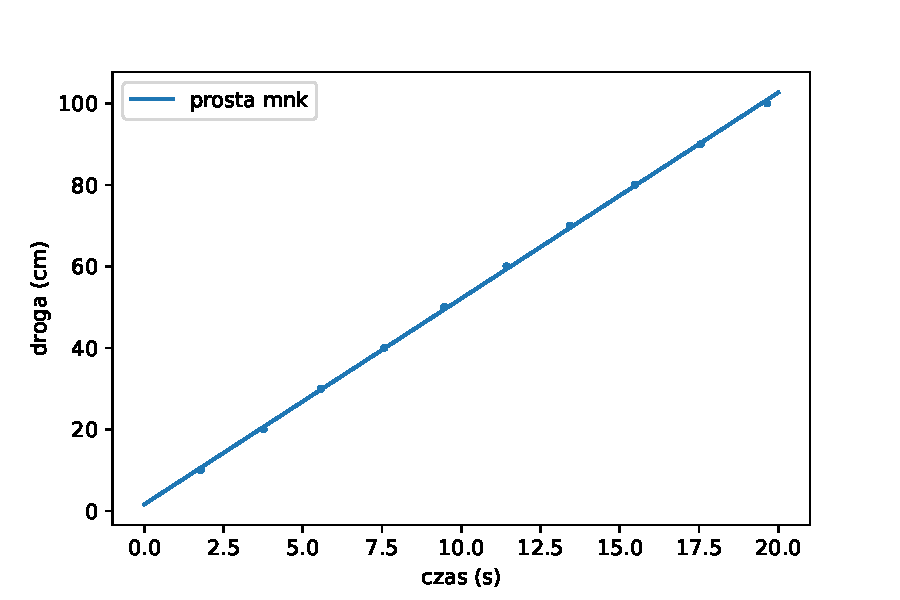
\includegraphics[scale=0.7]{regresja_gliceryna.pdf}
\caption{Wyliczona prosta regresji liniowej zestawiona wraz z uśrednioną drogą przebytą w czasie przez kulkę w glicerynie.}
\label{wykres_gliceryna}
\end{figure}

Niepewność tej wartości:

\begin{align*}
	u(\vgr) &= \sqrt{\left(\frac{\partial \vgr}{\partial h}\right)^2 u^2(h) + \left(\frac{\partial \vgr}{\partial t}\right)^2 u^2(t)} \\
	&= \sqrt{\frac{u^2(h)}{t^2} + \frac{h^2 u^2(t)}{t^4}} \\
	&\approx 0.305392770313 \, \frac{\text{cm}}{\text{s}} \\
	&\approx 0.31 \, \frac{\text{cm}}{\text{s}}
\end{align*}

Do wyliczenia niepewności do równania \ref{eq_lepkosc} potrzebne jeszcze będą nastepujące pochodne cząstkowe:

\begin{itemize}
	\item $\frac{\partial \eta}{\partial r} \approx \frac{g h r R (b (-0.0925926 h r - 0.0771605 h R - 0.119599 r R) + a (0.0925926 h r + 0.0771605 h R + 0.119599 r R))}{\vgr (h + 3.1r)^2 (r + 0.416667 R)^2}$;
	\item $\frac{\partial \eta}{\partial \vgr} \approx \frac{-0.0925926(\rho_k - \rho_c) g h r^2 R}{\vgr^2 (h + 3.1r)(r + 0.416667R)}$;
	\item $\frac{\partial \eta}{\partial R} \approx \frac{0.0925926(\rho_k - \rho_c) g h r^3}{\vgr (h + 3.1r)(r + 0.416667 R)^2}$;
	\item $\frac{\partial \eta}{\partial h} \approx \frac{0.287037 g r^3 R (\rho_k - \rho_c)}{v(h + 3.1r)^2 (r + 0.416667 R)}$.
\end{itemize}

Zatem, dla gliceryny:

\begin{align*}
	u(\eta) &= \sqrt{
	  \left(\frac{\partial \eta}{\partial r}\right)^2 u^2(r)
	+ \left(\frac{\partial \eta}{\partial \vgr}\right)^2 u^2(\vgr)
	+ \left(\frac{\partial \eta}{\partial R}\right)^2 u^2(R)
	+ \left(\frac{\partial \eta}{\partial h}\right)^2 u^2(h)
	} \\
	&\approx 0.029171820 \, \text{Pa s}\\
	&\approx 0.03 \, \text{Pa s}
\end{align*}

Korzystając z równania \ref{eq_lepkosc} mamy (dla gliceryny): $\eta \approx 0.47377301330 \, \text{Pa s} \approx 0.47 \, \text {Pa s}$.

\subsection{Wyznaczenie współczynnika lepkości oleju silnikowego}

Wyznaczenie współczynnika lepkości oleju silnikowego przebiegało w sposób analogiczny.
Należy do obliczeń użyć innej wartości prędkości granicznej poruszania się kulki w cieczy oraz gęstości cieczy.
Wartości pozostałych parametrów są takie same.

Za gęstość oleju silnikowego w warunkach laboratoryjnych przyjęliśmy wartość $\rho_\text{olej} = 0.867 \, \frac{\text{g}}{\text{cm}^3}$.

W tabeli \ref{olej} przedstawione zostały sumaryczne czasy wraz z międzyczasami.

\begin{table}[h!]
	\centering
	\begin{tabular}{lrrrrrrrrrrr}
		\toprule
		L.p. &  \#1 &  \#2 &  \#3 &  \#4 &  \#5 &  \#6 &  \#7 &  \#8 &  \#9 &  \#10 & suma (s)\\
		\midrule
		1 &           0.94 &           1.00 &           0.94 &           0.91 &           0.94 &           0.88 &           1.07 &           0.96 &           0.97 &            1.06 & 9.67 \\
		2 &           1.14 &           0.71 &           0.92 &           1.00 &           0.99 &           0.91 &           0.97 &           0.97 &           1.01 &            1.01 & 9.63 \\
		3 &           0.92 &           0.97 &           0.91 &           0.95 &           1.09 &           0.86 &           0.95 &           1.07 &           0.90 &            1.10 & 9.72 \\
		4 &           1.14 &           0.77 &           0.98 &           0.95 &           0.84 &           1.04 &           0.91 &           1.01 &           1.00 &            1.08 & 9.72 \\
		5 &           0.83 &           0.98 &           0.88 &           1.02 &           1.00 &           0.96 &           0.92 &           0.97 &           0.96 &            0.96 & 9.48 \\
		\bottomrule
		\end{tabular}
	\caption{Międzyczasy (s) pięciokrotnego pomiaru spadku kulki w oleju silnikowym.}
	\label{olej}
\end{table}

Zatem niepewność standardowa typu B pozostaje taka sama, $u_b(t) = 0.35$.

Przez $t_1, \dots, t_5$ oznaczmy kolejne sumaryczne czasy spadku.
Średni sumaryczny czas spadku wynosi $t = \frac 1 5 (t_1 + \dots + t_5) = 9.644 \approx 9.64$ s.
Ponadto, niepewność typu A pomiaru czasu wynosi:

\begin{align*}
	u_a(t) &= \sqrt{S^{2}_{\overline{t}}} \\
	&= \sqrt{\frac{1}{5 \cdot 4} \cdot \sum_{i=1}^{5} (t_i - t)^2} \\
	&\approx 0.04433959 \, \text{s} \\
	&\approx 0.05 \, \text{s}
\end{align*}

Ostatecznie niepewność czasu spadku wynosi $u(t) = \sqrt{u_a^2(t) + u_b^2(t)} = \sqrt{0.05^2 + 0.35^2} \, \text{s} \approx 0.35355339 \, \text{s} \approx 0.36\, \text{s}$.

Ponownie przyjęliśmy, że przed wkroczeniem na odcinek pomiarowy kulka osiągnęła prędkość graniczną.
Używając metody najmniejszych kwadratów, wyznaczyliśmy prostą regresji.
Dane zostały zaprezentowane na wykresie \ref{wykres_olej}.
Wartość współczynnika kierunkowego jest wartością graniczną prędkości, tzn.
$\vgr \approx 10.4028361 \, \frac{\text{cm}}{\text{s}} \approx 10.40 \, \frac{\text{cm}}{\text{s}}$.

\begin{figure}[h]
\centering
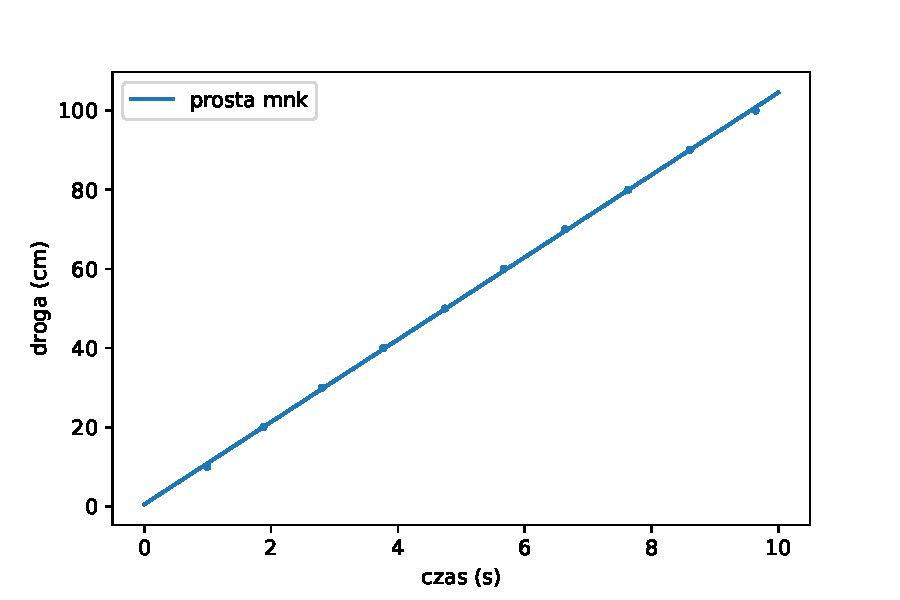
\includegraphics[scale=0.7]{regresja_olej.pdf}
\caption{Wyliczona prosta regresji liniowej zestawiona wraz z uśrednioną drogą przebytą w czasie przez kulkę w oleju.}
\label{wykres_olej}
\end{figure}

Niepewność tej wartości:

\begin{align*}
	u(\vgr) &= \sqrt{\left(\frac{\partial \vgr}{\partial h}\right)^2 u^2(h) + \left(\frac{\partial \vgr}{\partial t}\right)^2 u^2(t)} \\
	&= \sqrt{\frac{u^2(h)}{t^2} + \frac{h^2 u^2(t)}{t^4}} \\
	&\approx 0.387458073 \, \frac{\text{cm}}{\text{s}} \\
	&\approx 0.39 \, \frac{\text{cm}}{\text{s}}
\end{align*}

Licząc analogicznie współczynnik lepkości oraz jego niepewność -- analogicznie jak w przypadku gliceryny -- otrzymujemy:

$$
\eta = 0.24 (1) \, \text{Pa s}
$$

\subsection{Wnioski}

Warto zaznaczyć, że lepkość cieczy w dużym stopniu zależy od temperatury.
W celu nadania znaczenia wyliczonym wartościom lepkości, należałoby również wyznaczyć temperaturę cieczy podczas doświadczenia.

\end{document}
